% Current paper view. Historical control analyses remain in the r12 evidence archive.
\section{Experimental Evaluation}
\label{sec:experiments}

\subsection{Experimental Setup}
\subsubsection{Data and Evaluation Protocol}
We evaluate closed-set cross-receiver radio-frequency fingerprinting on the ManySig and ManyRx subsets of WiSig~\cite{wisig}. Source and target share the registered transmitter (TX) identities and have disjoint physical receiver (RX) sets. ManySig contains six TX, 12 RX and four acquisition dates: March 1, 8, 15 and 23, 2021 (D0--D3). We use equalized IQ, a central 256-sample window and float32 per-packet unit-RMS normalization before channel transformation, yielding a $2\times256$ input. Derived views of one packet retain its physical identity.

Table~\ref{tab:paper-data} lists the principal partitions. F0 has five source RX and seven target RX; its 15 source RX--date cells are not 15 physical receivers. F1/F2 change receiver membership while retaining the five/seven counts. For ManySig, packets ordered by stored physical indices within each source TX/RX/day cell are divided into 70 labeled training samples, 630 unlabeled samples and 300 validation samples. Thus L is 10\% of the training pool, while the additional source-validation labels are disclosed separately. U labels remain hidden. Validation updates no model or persistent state.

\begin{table*}[!t]
\centering\footnotesize
\caption{Principal data conditions. Receiver indices are dataset-local. F0/F1/F2 test all four dates; the chronological result uses future D3 only. Source and target are physically disjoint.}
\label{tab:paper-data}
\begin{tabular*}{\textwidth}{@{\extracolsep{\fill}}llccrr@{}}
\toprule
Condition & Source RX indices & Source/target RX & TX & $|L|/|U|/|V|$ & Test packets\\
\midrule
F0 & 1,3,4,6,8 & 5/7 & 6 & 6300/56700/27000 & 168000\\
F1 & 0,2,5,7,9 & 5/7 & 6 & 6300/56700/27000 & 168000\\
F2 & 1,3,4,10,11 & 5/7 & 6 & 6300/56700/27000 & 168000\\
Chronological & F0 source RX & 5/7 & 6 & 6300/56700/27000 & 42000 (D3)\\
ManyRx & Even indices 0--30 & 16/16 & 10 & 6533/58828/28023 & 123021\\
\bottomrule
\end{tabular*}
\end{table*}

F0/F1/F2 train on D1--D3 and test on all four dates. D0 is an earlier unseen date, not a future endpoint. The chronological setting trains on D0--D2 and evaluates the 42000 D3 packets from target RX. We do not label its all-date aggregate as future generalization. ManyRx contains missing and non-full cells, which are retained; its source roles use $\lfloor0.07n\rfloor$, $\lfloor0.63n\rfloor$ and the remainder per cell. ManySig and ManyRx share the WiSig acquisition system and are not independent capture campaigns.

Every test uses the same fixed received-IQ observations: clean plus high/mid/low suburban and high/mid/low urban synthetic channel conditions. These are simulated stress tests, not measured satellite-link validation. DURA is applied to every declared observation, including clean, without scene-aware bypass or additional output renormalization. Each model freezes every view and task before independent truth-side scoring. Target observations, labels and scores never enter training, hyperparameter selection, checkpoint selection or rerun decisions.

\subsubsection{Complete Baselines and PAMF Training}
We compare the complete methods RIEI~\cite{riei}, DRIFT-v2~\cite{drift}, IB-RFF~\cite{ibrff} and SDG~\cite{sdg}. Each retains its native objectives, jointly trained identity head and method-specific stopping rule (Table~\ref{tab:paper-budgets}). RIEI and DRIFT use the registered E100 implementation budgets; RIEI uses the registered short one-dimensional input stem. The comparison therefore evaluates complete recipes with their disclosed implementation budgets.

\begin{table*}[!t]
\centering\footnotesize
\caption{Registered training budgets and model selection. External semi-supervised variants add ordinary PL to the same complete method. PAMF-T1 uses its native selective self-training. No post-hoc classifier fitting is performed.}
\label{tab:paper-budgets}
\begin{tabular*}{\textwidth}{@{\extracolsep{\fill}}lp{0.36\textwidth}p{0.43\textwidth}@{}}
\toprule
Method & Budget and optimizer & Freeze and recipe\\
\midrule
RIEI & E100; batch 64; SGD $10^{-4}$ & Final epoch; three optimizer steps per batch for the complete objective.\\
DRIFT-v2 & E100; batch 256; Adam $10^{-4}$ & Final epoch; native adversarial, center and separation objectives.\\
IB-RFF & Two stages, each at most E200; batch 128; Adam $10^{-3}$ & Source-V minimum NLL; LR reduction patience 5; early-stop patience 10.\\
SDG & E200; batch 32; Adam $10^{-3}$ & Source-V minimum NLL; native two-view and contrastive objectives.\\
PAMF-Sup & E50/11100 updates; L batch 128; AdamW and segment cosine schedules & Fixed final checkpoint; supervised representation objectives; no U or EMA.\\
PAMF-T1 & E50/11100 updates; L batch 128, U batch 256; AdamW and segment cosine schedules & 13 labeled-only plus 37 joint epochs; own student/EMA inheritance across 20+10+20 stages.\\
\bottomrule
\end{tabular*}
\end{table*}

The complete external methods and PAMF-Sup use the registered clean-plus-satellite concatenation with satellite TX-CE weight 0.68 and no added satellite consistency loss. The augmentation probability is 0.30/0.60/0.80 over relative budget intervals $[0,.20)$, $[.20,.45)$ and $[.45,1)$. Weak clear, low-elevation and rain-named presets use the fixed simulator settings; the naming does not establish physical rain validation. Method-specific stopping can change realized augmentation exposure, especially for IB-RFF. Its two-stage early stopping and the corresponding source-only audit are retained.

External semi-supervised variants use current-model hard pseudo-labels at confidence 0.95, PL weight 1 and U/L batch ratio 1, without EMA, neighbor gates or strong-view consistency. RIEI runs with zero pseudo-label acceptance at the fixed threshold remain in the reported matrix; U exposure and realized acceptance are retained in the training records. PAMF-T1 retains the fixed native schedule: ordinary/raw stochastic consistency, shallow/intermediate cross-RX CRIC, As cross entropy with As KL disabled, label smoothing 0.01, and native selective U/EMA training. Student and own EMA states are inherited, while optimizers and segment schedules reset. A logical PAMF epoch contains 222 updates and need not equal one pass over a changed source pool.

\subsubsection{Restoration Permissions and Reporting}
F denotes the identifier and G the DURA restorer. Supervised system comparisons use G-L: every G ancestor trains using labeled-source IQ only, without consuming its TX labels. Semi-supervised system comparisons use G-LU, which may also consume TX-hidden source U. G training uses simulated source-IQ pairs, without F weights/outputs or target data. All ancestors match the classifier's source contract; a restorer from a different RX/date/TX split is not reused as a matching teacher. Restorer cost includes its source-only training ancestry and is shared across frozen F consumers.

We report Accuracy and Macro-F1 over the full registered class set (six classes for ManySig and ten for ManyRx). S6 averages the six channel conditions within each seed before computing mean and sample SD across F seeds 2026092701/02/03. Three F seeds usually share one fixed G per contract: the reported SD is conditional F variation, not three independent complete-system replicas or a significance interval. A separate preregistered three-source F/G crossed-seed study checks joint-seed sensitivity. The evidence archive includes per-RX/TX/day results and confusion-derived repair/damage counts.

\subsection{Comparison with Complete Methods}

\subsubsection{Supervised and Semi-Supervised Recognition}

Table~\ref{tab:full-f0} compares the four complete external methods with the corresponding PAMF recipe. The supervised block uses labeled-only F and same-contract G-L throughout. The semi-supervised block uses each external method with ordinary PL and PAMF-T1 with its native selective self-training, followed by G-LU. PAMF-Sup retains the registered supervised representation objectives and satellite augmentation but consumes no U or EMA; it is not the ordinary-PL control. PAMF-T1 is the fixed final method, not a relabeled PAMF-PL experiment.

\begin{table*}[!t]
\centering\footnotesize
\caption{F0 comparison of complete methods (\%). Raw applies F directly; restored applies the same-contract DURA before F. S6 is the within-seed six-scene mean. Entries are mean$\pm$sample SD over three F seeds.}
\label{tab:full-f0}
\begin{tabular*}{\textwidth}{@{\extracolsep{\fill}}lrrrrr@{}}
\toprule
Method & Raw clean & Raw S6 & Restored clean & Restored S6 & Restored S6 F1 \\
\midrule
\multicolumn{6}{@{}l}{\textit{Supervised F and G-L: labeled source IQ only}} \\
\addlinespace[2pt]
RIEI & \pmv{54.53}{8.31} & \pmv{47.68}{6.42} & \pmv{54.44}{8.24} & \pmv{49.33}{6.36} & \pmv{44.28}{9.42} \\
DRIFT-v2 & \pmv{67.33}{5.91} & \pmv{26.83}{3.36} & \pmv{67.22}{5.96} & \pmv{62.01}{6.30} & \pmv{61.09}{6.55} \\
IB-RFF & \pmv{63.77}{2.18} & \pmv{15.78}{4.87} & \pmv{63.83}{2.18} & \pmv{61.43}{1.98} & \pmv{60.41}{2.27} \\
SDG & \pmv{71.39}{1.84} & \pmv{58.14}{2.32} & \pmv{71.43}{1.85} & \pmv{65.22}{1.85} & \pmv{64.95}{1.49} \\
\textbf{PAMF-Sup} & \pmv{84.01}{0.94} & \pmv{70.08}{1.49} & \pmv{83.95}{0.98} & \pmv{76.84}{0.53} & \pmv{76.49}{0.71} \\
\addlinespace[4pt]
\multicolumn{6}{@{}l}{\textit{Semi-supervised F and G-LU: unlabeled source IQ allowed}} \\
\addlinespace[2pt]
RIEI & \pmv{53.53}{6.48} & \pmv{47.50}{5.66} & \pmv{53.53}{6.49} & \pmv{48.22}{4.86} & \pmv{43.21}{7.89} \\
DRIFT-v2 & \pmv{60.97}{11.26} & \pmv{27.28}{3.11} & \pmv{60.88}{11.31} & \pmv{56.57}{9.42} & \pmv{55.24}{11.36} \\
IB-RFF & \pmv{66.08}{0.99} & \pmv{18.44}{4.30} & \pmv{66.08}{0.96} & \pmv{63.66}{0.96} & \pmv{62.75}{0.63} \\
SDG & \pmv{72.10}{0.41} & \pmv{58.15}{1.53} & \pmv{72.08}{0.41} & \pmv{66.18}{0.21} & \pmv{66.44}{0.35} \\
\textbf{PAMF-T1} & \pmv{84.39}{0.92} & \pmv{70.60}{1.06} & \pmv{84.48}{0.97} & \pmv{77.65}{0.85} & \pmv{77.48}{0.87} \\
\bottomrule
\end{tabular*}
\end{table*}

On F0, PAMF-Sup reaches \pmv{76.84}{0.53}\% S6 accuracy, while PAMF-T1 reaches \pmv{77.65}{0.85}\%. Their respective raw S6 values are \pmv{70.08}{1.49}\% and \pmv{70.60}{1.06}\%. Table~\ref{tab:full-scenes} retains all seven conditions, including the difficult low-urban endpoint. These are complete-recipe comparisons with method-specific objectives and budgets; they do not isolate the effect of an individual SSL component.

\begin{table*}[!t]
\centering\footnotesize
\caption{Restored F0 accuracy on every declared condition (\%). S/U denote suburban/urban and H/M/L denote channel severity. Methods retain the same source and target roles within each setting.}
\label{tab:full-scenes}
\begin{tabular*}{\textwidth}{@{\extracolsep{\fill}}lrrrrrrr@{}}
\toprule
Method & Clean & S-H & S-M & S-L & U-H & U-M & U-L \\
\midrule
\multicolumn{8}{@{}l}{\textit{Supervised: DURA-L}} \\
\addlinespace[2pt]
RIEI & \pmv{54.44}{8.24} & \pmv{52.41}{7.12} & \pmv{51.33}{6.88} & \pmv{50.17}{6.49} & \pmv{51.45}{6.95} & \pmv{47.20}{5.81} & \pmv{43.44}{4.90} \\
DRIFT-v2 & \pmv{67.22}{5.96} & \pmv{65.25}{7.17} & \pmv{64.42}{6.79} & \pmv{63.31}{6.39} & \pmv{64.36}{6.90} & \pmv{59.72}{5.75} & \pmv{55.02}{4.82} \\
IB-RFF & \pmv{63.83}{2.18} & \pmv{63.20}{2.45} & \pmv{62.82}{2.23} & \pmv{62.41}{2.01} & \pmv{62.83}{2.40} & \pmv{60.25}{1.65} & \pmv{57.04}{1.15} \\
SDG & \pmv{71.43}{1.85} & \pmv{69.03}{1.66} & \pmv{67.94}{1.77} & \pmv{66.63}{1.96} & \pmv{67.96}{1.70} & \pmv{62.54}{1.96} & \pmv{57.24}{2.18} \\
\textbf{PAMF-Sup} & \pmv{83.95}{0.98} & \pmv{82.28}{0.76} & \pmv{80.69}{0.57} & \pmv{79.02}{0.51} & \pmv{80.70}{0.66} & \pmv{72.82}{0.45} & \pmv{65.51}{0.47} \\
\addlinespace[4pt]
\multicolumn{8}{@{}l}{\textit{Semi-supervised: DURA-LU}} \\
\addlinespace[2pt]
RIEI & \pmv{53.53}{6.49} & \pmv{50.80}{5.59} & \pmv{49.86}{5.38} & \pmv{48.81}{5.03} & \pmv{49.93}{5.31} & \pmv{46.53}{4.27} & \pmv{43.38}{3.60} \\
DRIFT-v2 & \pmv{60.88}{11.31} & \pmv{59.66}{10.47} & \pmv{58.41}{10.10} & \pmv{56.88}{9.72} & \pmv{59.01}{10.20} & \pmv{54.71}{8.66} & \pmv{50.75}{7.40} \\
IB-RFF & \pmv{66.08}{0.96} & \pmv{65.28}{1.18} & \pmv{64.86}{1.07} & \pmv{64.36}{0.92} & \pmv{65.03}{1.14} & \pmv{62.75}{0.88} & \pmv{59.70}{0.65} \\
SDG & \pmv{72.08}{0.41} & \pmv{70.01}{0.42} & \pmv{68.71}{0.28} & \pmv{67.32}{0.23} & \pmv{68.99}{0.34} & \pmv{63.51}{0.05} & \pmv{58.54}{0.07} \\
\textbf{PAMF-T1} & \pmv{84.48}{0.97} & \pmv{82.30}{0.87} & \pmv{81.00}{0.89} & \pmv{79.47}{0.87} & \pmv{81.06}{0.95} & \pmv{74.40}{0.81} & \pmv{67.66}{0.71} \\
\bottomrule
\end{tabular*}
\end{table*}

\begin{figure*}[!t]\centering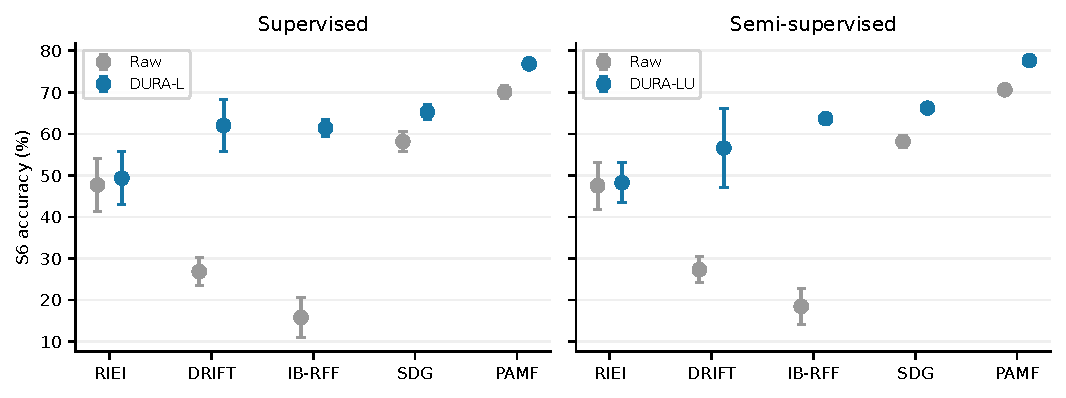
\includegraphics[width=.94\textwidth]{images/full_methods/f0_complete.pdf}\caption{Complete external methods and the corresponding PAMF recipe on F0. Raw and restored S6 accuracy use the same frozen F in each comparison. Error bars are three-F-seed sample SD.}\label{fig:full-f0}\end{figure*}

Restoration does not uniformly improve clean observations or every external classifier. For example, F0 IB-RFF in the supervised setting has S6 accuracy \pmv{61.43}{1.98}\% with G-L, compared with \pmv{15.78}{4.87}\% on raw input; RIEI changes from \pmv{47.68}{6.42}\% to \pmv{49.33}{6.36}\%. All clean reductions and nonmonotonic results remain in the tables and curves. We do not choose the restoration route or bypass from the true test condition.

\subsubsection{Receiver, Date and Label Generalization}

Table~\ref{tab:full-generalization} retains the available complete supervised methods across receiver partitions, the larger TX/RX setting and the future-date endpoint. External semi-supervised models exist for F0 and the natural source-count suite; untrained external SSL cells are not invented for these other conditions. The low-label comparison in Table~\ref{tab:full-labels} includes only the registered IB-RFF and PAMF-Sup models.

\begin{table*}[!t]
\centering\footnotesize
\caption{Supervised generalization with G-L (S6 accuracy, \%). F1/F2 use alternate disjoint RX partitions. ManyRx has ten classes. Chronological evaluation uses target RX on D3 only (42000 packets), not the all-date aggregate.}
\label{tab:full-generalization}
\begin{tabular*}{\textwidth}{@{\extracolsep{\fill}}lrrrr@{}}
\toprule
Method & F1 & F2 & ManyRx & Future D3 \\
\midrule
RIEI & \pmv{56.12}{0.81} & \pmv{59.02}{0.56} & \pmv{26.62}{6.45} & \pmv{52.59}{3.45} \\
DRIFT-v2 & \pmv{56.65}{3.18} & \pmv{61.47}{1.70} & \pmv{40.30}{4.19} & \pmv{60.38}{4.99} \\
IB-RFF & \pmv{58.05}{0.97} & \pmv{60.35}{0.94} & \pmv{62.78}{1.00} & \pmv{68.18}{1.48} \\
SDG & \pmv{59.89}{0.73} & \pmv{64.83}{0.98} & \pmv{64.84}{0.50} & \pmv{70.06}{0.68} \\
\textbf{PAMF-Sup} & \pmv{65.44}{0.36} & \pmv{71.99}{0.63} & \pmv{71.49}{0.33} & \pmv{74.52}{2.36} \\
\bottomrule
\end{tabular*}
\end{table*}

\begin{table}[!t]
\centering\footnotesize
\caption{Label efficiency under full L-only systems (S6 accuracy, \%). Only IB-RFF has registered external low-label models. All rows use the same seven target RX and separate source-validation labels.}
\label{tab:full-labels}
\begin{tabular*}{\columnwidth}{@{\extracolsep{\fill}}lrr@{}}
\toprule
L fraction (\%) & IB-RFF & PAMF-Sup \\
\midrule
1 & \pmv{60.72}{1.49} & \pmv{69.73}{0.46} \\
5 & \pmv{64.05}{1.72} & \pmv{74.29}{0.84} \\
10 & \pmv{61.43}{1.98} & \pmv{76.84}{0.53} \\
\bottomrule
\end{tabular*}
\end{table}

\subsubsection{Source-Receiver Diversity}

Figure~\ref{fig:full-source} compares the five complete methods using exactly six target RX/144000 packets at every point. Natural budgets use $(|L|,|U|,|V|)=(1260m,11340m,5400m)$; the fixed-L/V supervised setting uses $(1080,12600m-1080,5400)$ with no U consumed. The source counts are $m=1,2,3,4,6$. F0 uses seven target RX/168000 packets and is not inserted as an $m=5$ point. A single source RX provides no cross-RX positive pair, so the corresponding PAMF contrast term has zero valid-anchor coverage. Natural SSL curves vary both receiver diversity and available U; they do not isolate receiver count alone.

\begin{figure*}[!t]\centering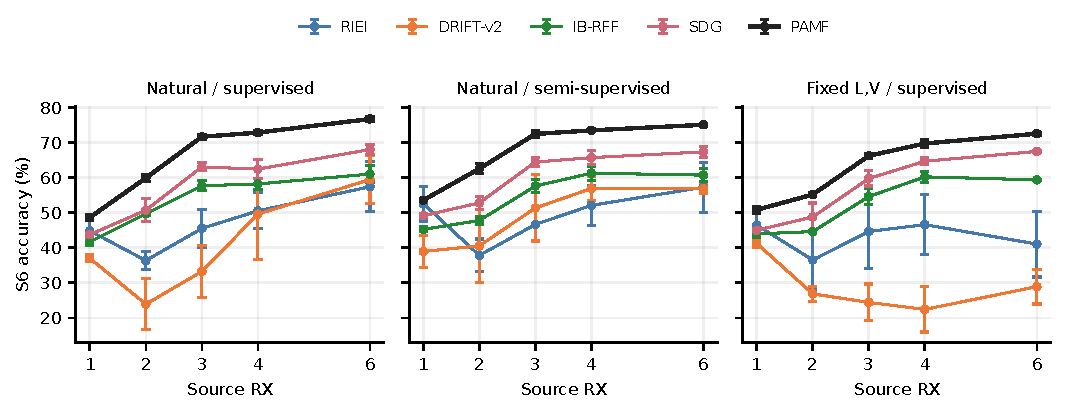
\includegraphics[width=\textwidth]{images/full_methods/source_complete.pdf}\caption{Source-count comparison using complete external methods and PAMF. Supervised panels use G-L; the semi-supervised panel uses G-LU. Each line retains its registered training budget, three F seeds, all negative effects and nonmonotonicity. The fixed-L/V panel controls annotation count.}\label{fig:full-source}\end{figure*}

The source curves provide a broader view than the F0 endpoint: increasing source RX does not guarantee monotonic gains, and PAMF is not assumed to dominate every low-source condition. The source-validation stopping rules remain fixed; test results never select an epoch, branch, seed or rerun.


\subsection{PAMF Mechanism Analysis}

\subsubsection{Three Core Training Mechanisms}

We group the identification objectives by function rather than observed gain. A is CRIC: shallow/intermediate same-TX, cross-physical-RX contrast. B is stochastic prediction consistency: ordinary128, ordinary64 and raw128 symmetric-KL terms switch together. C is native selective self-training: own EMA, confidence and adjacent/strong-view gates, pseudo-label CE and U entropy switch together. Table~\ref{tab:paper-core} reports the complete model and one removal per group. Each removal retains the supervised CE dose and update schedule; C-off performs no U loading or EMA work.

\begin{table*}[!t]
\centering\footnotesize
\caption{PAMF core-group ablation on F0 (accuracy, \%). All restored rows use fixed G-LU; C-off removes U from F only.}
\label{tab:paper-core}
\begin{tabular*}{\textwidth}{@{\extracolsep{\fill}}lrrrr@{}}
\toprule
F training setting & Raw clean & Raw S6 & DURA clean & DURA S6 \\
\midrule
Full PAMF-T1 & \pmv{84.39}{0.92} & \pmv{70.60}{1.06} & \pmv{84.48}{0.97} & \pmv{77.65}{0.85} \\
Without A: CRIC & \pmv{84.73}{0.51} & \pmv{70.99}{1.24} & \pmv{84.78}{0.58} & \pmv{78.06}{0.48} \\
Without B: consistency & \pmv{83.14}{0.76} & \pmv{70.50}{0.61} & \pmv{83.13}{0.82} & \pmv{76.63}{0.48} \\
Without C: selective SSL & \pmv{84.79}{0.82} & \pmv{70.60}{0.95} & \pmv{84.86}{0.87} & \pmv{77.85}{0.40} \\
\bottomrule
\end{tabular*}
\end{table*}

B increases raw clean accuracy by $1.25\pm1.09$ pp and restored S6 by $1.01\pm0.80$ pp in the complete combination. A and C have negative mean conditional restored-S6 differences ($-0.41\pm0.38$ and $-0.21\pm0.58$ pp for full minus removal). The data therefore do not support a claim that all three groups yield stable positive gains in this fixed F0 setting. These results retain the designated default and are not used to regroup objectives or select reruns. The complete eight-combination diagnostic is retained in the experiment archive rather than expanded into the main comparison.

\subsubsection{Physical Structure and Inductive Bias}

Table~\ref{tab:paper-structure} isolates architecture under a common labeled-only objective. The single SIG\_TIME variant changes the number of learned views; branch deletions change capacity and computation. No-time, covariance, shuffled-time and scrambled-reference controls retain parameter count but change representation or input structure. They distinguish useful response/statistical features from a claim that a specific coordinate ordering is indispensable.

\begin{table*}[!t]
\centering\footnotesize
\caption{Physical-structure ablation under matched labeled-only CE plus satellite augmentation: no CRIC/KL/EMA/U, 11100 updates (accuracy, \%). The full PAMF-Sup recipe is evaluated separately.}
\label{tab:paper-structure}
\begin{tabular*}{\textwidth}{@{\extracolsep{\fill}}lrrrr@{}}
\toprule
PAMF backbone & Raw clean & Raw S6 & G-L S6 & G-L S6 F1 \\
\midrule
Full X3 backbone & \pmv{81.55}{1.34} & \pmv{46.35}{1.74} & \pmv{74.49}{1.14} & \pmv{73.91}{1.29} \\
Single SIG\_TIME & \pmv{81.82}{1.26} & \pmv{43.61}{6.18} & \pmv{74.20}{1.16} & \pmv{73.72}{1.33} \\
Without time coordinate & \pmv{80.95}{1.54} & \pmv{45.46}{5.89} & \pmv{73.99}{1.03} & \pmv{73.39}{1.27} \\
Without signature branch & \pmv{79.48}{1.72} & \pmv{41.84}{5.75} & \pmv{72.32}{1.09} & \pmv{71.92}{1.09} \\
Without PA branch & \pmv{78.94}{2.29} & \pmv{39.39}{5.78} & \pmv{71.70}{0.44} & \pmv{71.13}{0.49} \\
Without reference response & \pmv{78.64}{1.49} & \pmv{44.80}{2.93} & \pmv{73.01}{1.15} & \pmv{72.32}{1.16} \\
Covariance X3 & \pmv{81.69}{0.61} & \pmv{49.36}{4.72} & \pmv{74.56}{0.84} & \pmv{73.89}{0.89} \\
Shuffled time & \pmv{82.20}{1.72} & \pmv{48.54}{6.44} & \pmv{75.62}{1.11} & \pmv{75.10}{1.24} \\
Scrambled reference & \pmv{81.02}{1.20} & \pmv{46.59}{2.91} & \pmv{74.24}{1.09} & \pmv{73.64}{1.24} \\
\bottomrule
\end{tabular*}
\end{table*}

Removing PA, signature or reference-response features reduces G-L S6 accuracy relative to the full backbone by $2.79\pm0.86$, $2.17\pm0.11$ and $1.48\pm0.01$ pp. However, shuffled time exceeds the original ordering after restoration, and covariance X3 is slightly higher on average. These counterexamples are retained: physical structure supplies an inductive bias, not a guarantee that every chosen coordinate or prior is optimal.

The frozen source diagnostics use the same 720 labeled packets from 90 TX/RX/day strata and 11 fixed interventions. They access neither U nor target data and fit no probe. For full T1, same-TX cross-RX feature distance is $0.0618\pm0.0105$, compared with $0.0685\pm0.0118$ without A, while the separation margin does not increase. Lower within-identity distance alone does not establish complete receiver/channel disentanglement. Simulated PA interventions test sensitivity and are not assumed to preserve unknown hardware identity.

\subsubsection{Restoration Mechanisms}

Table~\ref{tab:paper-G} retains the coarse restoration, conjugate-gradient solver, conjugate-image action and residual-input controls that directly describe DURA. All use frozen T1 default heads, identical seven-view observations and source-only G training. Coarse restoration alone is insufficient; removing CG, image action or residual input also reduces the restored S6 mean. Initialization and distillation diagnostics remain in the archive and do not occupy a separate external-comparator analysis.

\begin{table*}[!t]
\centering\footnotesize
\caption{DURA functional ablation (accuracy, \%). Default: three F seeds with one G; other rows: same-index F/G students. SD describes the respective seed design.}
\label{tab:paper-G}
\begin{tabular*}{\textwidth}{@{\extracolsep{\fill}}lrrrr@{}}
\toprule
Restorer & Parameters (K) & Clean & S6 & Low urban \\
\midrule
Default DURA & 267.0 & \pmv{84.48}{0.97} & \pmv{77.65}{0.85} & \pmv{67.66}{0.71} \\
Coarse only & 106.1 & \pmv{83.26}{1.02} & \pmv{72.11}{0.77} & \pmv{55.95}{1.24} \\
Without CG & 267.0 & \pmv{84.41}{1.08} & \pmv{76.94}{1.08} & \pmv{66.45}{1.31} \\
Without image action & 267.0 & \pmv{84.49}{0.96} & \pmv{77.32}{1.10} & \pmv{67.09}{1.38} \\
Without residual input & 267.0 & \pmv{84.38}{0.94} & \pmv{76.78}{1.21} & \pmv{66.65}{1.53} \\
\bottomrule
\end{tabular*}
\end{table*}


\subsection{Computational Efficiency}

All inference measurements use frozen seed01 weights, FP32 with TF32 disabled, two CPU threads and exclusive RTX3090 access. Five measurement rounds describe timing variation, not five model seeds. Table~\ref{tab:paper-latency} includes complete external identifiers F, the proposed identifier and the restoration components. The external F-only measurements do not establish their online G+F latency; cached classification time is not substituted for it. The default PAMF F+G route has GPU-wall median $4.541$ms and P95 $4.725$ms; CPU class return has median $4.611$ms. The same weights take $37.190$ms on the native execution path, giving an $8.189\times$ execution-route improvement. This is not a claim that every external model received identical implementation optimization.

\begin{table*}[!t]\centering\footnotesize
\caption{Inference on RTX3090 (ms, five rounds). (a) Batch-one GPU wall and CPU-return latency; external F is eager, online external G+F is unmeasured. (b) PAMF F+G throughput in 256-sample IQ windows/s.}
\label{tab:paper-latency}
\begin{minipage}[t]{.71\textwidth}\centering
\textit{(a) Batch-one latency}\\[4pt]
\setlength{\tabcolsep}{3pt}
\begin{tabular*}{\linewidth}{@{\extracolsep{\fill}}llrrr@{}}\toprule
Model & Execution & Median & P95 & CPU return \\ \midrule
RIEI F & Eager & 2.352 & 2.734 & 2.456 \\
DRIFT-v2 F & Eager & 2.408 & 2.605 & 2.476 \\
IB-RFF F & Eager & 1.456 & 2.168 & 1.506 \\
SDG F & Eager & 3.054 & 5.008 & 3.105 \\
PAMF-T1 F & CUDA Graph & 0.757 & 0.858 & 0.796 \\
DURA G & Graph + residual reuse & 3.843 & 3.984 & 3.874 \\
PAMF-T1 F+G & Graph + residual reuse & 4.541 & 4.725 & 4.611 \\
\bottomrule\end{tabular*}\end{minipage}\hfill
\begin{minipage}[t]{.27\textwidth}\centering
\textit{(b) Batch throughput}\\[4pt]
\setlength{\tabcolsep}{3pt}
\begin{tabular*}{\linewidth}{@{\extracolsep{\fill}}rrr@{}}\toprule
Batch & Median & IQ/s \\ \midrule
1 & 4.541 & 220.2 \\
8 & 13.747 & 581.9 \\
32 & 28.374 & 1127.8 \\
64 & 15.295 & 4184.5 \\
128 & 17.111 & 7480.5 \\
\bottomrule\end{tabular*}\end{minipage}
\end{table*}

F and G contain 232993 and 266951 registered learned parameters (499944 total). Separate eager Conv/Linear profiles give 8.856M and 25.068M real MACs; these omit functional-head arithmetic, FFT complex operations, CG reductions and elementwise work, so they are not total FLOPs. Eager G uses 43 FFT/IFFT calls; the residual-reuse route uses 27. The larger training wrapper, optimizer and EMA are not counted as deployment parameters. Multi-model/Graph resident allocation is not reported as single-model VRAM.

Table~\ref{tab:paper-latency}(b) preserves the nonmonotonic batch latency. Amortized throughput does not establish continuous full-rate radio operation. Training-only CRIC, stochastic forwards, EMA and U gates add no deployment passes. Source-stage cost, G ancestry, cached inference and scoring costs are reported separately in the evidence archive.

